\section{More Experimental Details and Results}

In this section, we report more experimental details and results. 
We present the details of adopted DG datasets, including PACS, VLCS, OfficeHome, TerraInc, DomainNet, and NICO++, for our evaluation, in \ref{sec:datasets}.
We present the training details and hyperparameter search space in \ref{sec:training_details}.
We present the detailed results of current optimizers on DG datasets in \ref{sec:results_of_opts}. We report more results of current optimizers ensembled with DG methods in \ref{sec:ensemble}. We report the detailed results of models trained with current optimizers and FAD for various training iterations in \ref{sec:various_iter}. 




\subsection{Datasets}
\label{sec:datasets}

In this subsection, we introduce DG datasets in current benchmarks, including PACS, VLCS, OfficeHome, TerralInc, DomainNet, and NICO++.

\textbf{PACS} \cite{li2017deeper} is a widely used benchmark for domain generalization. It consists of 7 object categories spanning 4 image styles, namely \textsl{photo, art-painting, cartoon}, and \textsl{sketch}. We adopt the protocol in \cite{li2017deeper} to split the training and validation set.

\textbf{VLCS} \cite{fang2013unbiased} consists of 5 object categories shared by the PASCAL VOC 2007, LabelMe, Caltech and Sun datasets. We follow the standard protocol of \cite{ghifary2015domain} and divide each domain into a training set (70\%) and validation set (30\%) randomly. 

\textbf{OfficeHome} \cite{venkateswara2017deep} includes 65 categories and 4 domains, namely \textsl{art, clipart, product}, and \textsl{real}. It contains 15,588 samples.

\textbf{Terra Incognita} \cite{beery2018recognition} contains photographs of wild animals shot at 4 locations, namely L100, L38, L43, and L46. We adopt the subset of it used in DomainBed\cite{gulrajani2020search} and it consists of 10 categories and 24,788 samples.

\textbf{DomainNet} \cite{peng2019moment} contains 6 domains, including \textsl{clipart, infograph, painting, quickdraw, real}, and \textsl{sketch}. It contains 345 categories and 586,575 samples. 

\textbf{NICO++} \cite{zhang2022nico++} is a large scale OOD dataset. It contains more than 200,000 natural images. It consists of 80 categories and 10 common contexts for DG tasks.



\subsection{Training details}
\label{sec:training_details}
As introduced in Section Experiments, we follow the basic training and evaluation protocol introduced in \cite{gulrajani2020search}, where the information of test data is unavailable for hyperparameter search. 
We train all the models on DomainNet for 15,000 iterations as suggested in \cite{cha2021swad}, 10,000 iterations on NICO++, and 5,000 iterations on other datasets unless otherwise noted. 
For datasets except for NICO++, we follow the leave-one-out protocol in \cite{gulrajani2020search} where one domain is chosen as the target domain and the remaining domains as the training domain.
For NICO++, we choose two domains as target domains in each run and train models on the remaining four domains. Following the official combination \cite{zhang2022nico++}, we select \{\textit{autumn
}, \textit{rock}\}, \{\textit{dim},\textit{grass}\}, \{\textit{outdoor}, \textit{water}\} as the target domain pairs. Detailed training and test splits of NICO++ are shown in Table \ref{tab:nico_split}. We use the official training subset of each selected training domain for training and test subset for test. We report the results of all the domains together in Table \ref{tab:nico10k}.

\begin{table*}[th]
\centering
\caption{The detailed split of training and test domains of NICO++.}
\begin{tabular}{l|c}
\toprule
Training domains & Test domains \\
\midrule
  dim, grass, outdoor, water & autumn, rock \\ 
 autumn, rock, outdoor, water & dim, grass \\
autumn, rock, dim, grass &  outdoor, water \\

\bottomrule
\end{tabular}
\label{tab:nico_split}
\end{table*}

All the models are evaluated following the protocol in DomainBed. The search space of hyperparameters is shown in Table \ref{tab:hyper_space}.

\begin{table*}[th]
\centering
\caption{The search space of hyperparameters.}
\begin{tabular}{l|cc}
\toprule
Parameter & Default value & Search Distribution \\
\midrule
batch size & 32 & 2$^{\rm Uniform(3, 5.5)}$ \\
learning rate & 0.00005 & 10$^{\rm Uniform(-5, -3.5)}$ \\
momentum & 0.9 & 10$^{\rm Uniform(-1, 0)}$ \\
weight decay & 0.0001 & 10$^{\rm Uniform(-6, -3)}$ \\
\bottomrule
\end{tabular}
\label{tab:hyper_space}
\end{table*}

For the search space of algorithm-specific hyperparameters of SAM \cite{du2021efficient} and GAM \cite{Zhang2023GradientNA}, we follow the settings in their original papers, where $\rho$ is searched in \{0.01, 0.05, 0.1, 0.2, 0.5, 1.0\} and $\alpha$ in \{0.1, 0.2, 0.5, 1.0, 2.0, 3.0, ..., 10.0\}. There are three unique hyperparameters in GAM, namely $\rho$, $\alpha$, and $\beta$. We search $\rho$ in \{0.05, 0.1, 0.2, 0.5, 1.0, 2.0\}, $\alpha$ in \{0.1, 0.2, ..., 1.0\}, and $\beta$ in \{0.01, 0.05, 0.1, 0.2, 0.5, 1.0\}. Please note that all the hyperparameters are randomly selected following the protocol in DomainBed and no information of test data is known in the training and model selection phase. For SAM, GAM, and FAD, we use SGD, which is the naive optimizer compared with adaptive or second-order aware optimizers, and the base optimizer.      

\subsection{Detailed results of current optimizers on DG datasets with the evaluation protocol in DomainBed.}
\label{sec:results_of_opts}
We report the test accuracy of current optimizers and FAD on different target domains of DG datasets.  

\subsubsection{PACS}
We report the detailed results on PACS in Table \ref{tab:pacs5k}. FAD consistently outperforms its counterparts on all domains.
\begin{table*}[th]
\centering
\caption{The comparison of optimizers on PACS. All the models are trained for 5,000 iterations and evaluated following the protocol in DomainBed~\cite{gulrajani2020search}. The best results for each domain are highlighted in bold font.}
\begin{tabular}{lcccc|c}
\toprule
\textbf{Algorithm} & art & cartoon & photo & sketch  & \textbf{Avg.} \\
\midrule

Adam  & 88.0 \footnotesize{$\pm 1.2$} &  79.7 \footnotesize{$\pm 0.5$} & 96.7 \footnotesize{$\pm 0.4$} & 72.7 \footnotesize{$\pm 0.9$} & 84.3 \\
AdamW  & 84.1 \footnotesize{$\pm 1.5$} & 80.7 \footnotesize{$\pm 1.2$}  & 96.9 \footnotesize{$\pm 0.4$} & 72.8 \footnotesize{$\pm 0.6$} & 83.6 \\
SGD  & 85.1 \footnotesize{$\pm 0.4$} & 76.0 \footnotesize{$\pm 0.3$}  & 98.3 \footnotesize{$\pm 0.4$} & 60.3 \footnotesize{$\pm 6.1$} & 79.9 \\
YOGI  & 84.4 \footnotesize{$\pm 1.7$} & 79.7 \footnotesize{$\pm 0.6$}  & 95.8 \footnotesize{$\pm 0.3$} & 65.1 \footnotesize{$\pm 1.5$} & 81.2 \\
AdaBelief  & 85.4 \footnotesize{$\pm 2.2$} & 80.4 \footnotesize{$\pm 1.1$}  & 97.4 \footnotesize{$\pm 0.7$} & 75.1 \footnotesize{$\pm 1.4$} & 84.6\\
AdaHessian  & 88.4 \footnotesize{$\pm 0.6$} &  80.0 \footnotesize{$\pm 0.9$} & 97.7 \footnotesize{$\pm 0.4$} & 71.7 \footnotesize{$\pm 4.1$} & 84.5 \\
SAM  & 85.7 \footnotesize{$\pm 1.2$} & 81.0 \footnotesize{$\pm 1.4$}  & 97.1 \footnotesize{$\pm 0.2$} & 77.4 \footnotesize{$\pm 1.8$} & 85.3 \\
GAM  & 85.9 \footnotesize{$\pm 0.9$} & 81.3 \footnotesize{$\pm 1.6$}  & 98.2 \footnotesize{$\pm 0.4$} & 79.0 \footnotesize{$\pm 2.1$} & 86.1 \\
\midrule
FAD (ours)  & \textbf{88.5} \footnotesize{$\pm 0.5$} & \textbf{83.0} \footnotesize{$\pm 0.8$}  & \textbf{98.4} \footnotesize{$\pm 0.2$} & \textbf{82.8} \footnotesize{$\pm 0.9$} & \textbf{88.2} \\

\bottomrule
\end{tabular}
\label{tab:pacs5k}
\end{table*}


\subsubsection{VLCS}
We report the detailed results on VLCS in Table \ref{tab:vlcs5k}. FAD outperforms its counterparts on 3 out of 4 domains and achieves the highest average accuracy.

\begin{table*}[th]
\centering
\caption{The comparison of optimizers on VLCS. All the models are trained for 5,000 iterations and evaluated following the protocol in DomainBed~\cite{gulrajani2020search}. The best results for each domain are highlighted in bold font.}
\begin{tabular}{lcccc|c}
\toprule
\textbf{Algorithm} & Caltech & LabelMe & SUN & VOC  & \textbf{Avg.} \\
\midrule

Adam & 98.9 \footnotesize{$\pm 0.4$} &  65.9 \footnotesize{$\pm 1.5$} & 71.0 \footnotesize{$\pm 1.6$} & 74.5 \footnotesize{$\pm 2.0$} & 77.3 \\
AdamW  & 98.3 \footnotesize{$\pm 0.1$} &  65.1 \footnotesize{$\pm 1.7$} & 70.9 \footnotesize{$\pm 1.3$} & 75.2 \footnotesize{$\pm 1.5$} & 77.4 \\
SGD  & 98.4 \footnotesize{$\pm 0.2$} &  64.7 \footnotesize{$\pm 0.7$} & 72.5 \footnotesize{$\pm 0.8$} & 76.6 \footnotesize{$\pm 0.8$} & 78.1 \\
YOGI  & 98.1 \footnotesize{$\pm 0.7$} &  63.9 \footnotesize{$\pm 1.2$} & 72.5 \footnotesize{$\pm 1.6$} & 75.7 \footnotesize{$\pm 1.2$} & 77.6 \\
AdaBelief  & 98.0 \footnotesize{$\pm 0.1$} &  63.9 \footnotesize{$\pm 0.4$} & 73.4 \footnotesize{$\pm 1.0$} & \textbf{78.2} \footnotesize{$\pm 1.8$} & 78.4 \\
AdaHessian  & \textbf{99.1} \footnotesize{$\pm 0.3$} &  65.0 \footnotesize{$\pm 1.7$} & 72.7 \footnotesize{$\pm 1.3$} & 77.7 \footnotesize{$\pm 1.0$} & 78.6 \\
SAM  & 98.5 \footnotesize{$\pm 1.0$} & 66.2 \footnotesize{$\pm 1.6$}  & 72.0 \footnotesize{$\pm 1.0$} & 76.1 \footnotesize{$\pm 1.0$} &  78.2 \\
GAM  & 98.8 \footnotesize{$\pm 0.6$} & 65.1 \footnotesize{$\pm 1.2$}  & 72.9 \footnotesize{$\pm 1.0$} & 77.2 \footnotesize{$\pm 1.9$} & 78.5 \\
\midrule
FAD (ours)  & \textbf{99.1} \footnotesize{$\pm 0.5$} & \textbf{66.8} \footnotesize{$\pm 0.9 $}  & \textbf{73.6} \footnotesize{$\pm 1.0 $} & 76.1 \footnotesize{$\pm 1.3$} &  \textbf{78.9} \\

\bottomrule
\end{tabular}
\label{tab:vlcs5k}
\end{table*}


\subsubsection{OfficeHome}
We report the detailed results on OfficeHome in Table \ref{tab:office5k}. FAD outperforms its counterparts on 3 out of 4 domains and achieves the highest average accuracy.
\begin{table*}[th]
\centering
\caption{The comparison of optimizers on OfficeHome. All the models are trained for 5,000 iterations and evaluated following the protocol in DomainBed~\cite{gulrajani2020search}. The best results for each domain are highlighted in bold font.}
\begin{tabular}{lcccc|c}
\toprule
\textbf{Algorithm} & Art & Clipart & Product & Real-World  & \textbf{Avg.} \\
\midrule

Adam  & 63.9 \footnotesize{$\pm 0.8$} & 48.1 \footnotesize{$\pm 0.6$} & 77.0 \footnotesize{$\pm 0.9$} & 81.8 \footnotesize{$\pm 1.6$} & 67.6 \\
AdamW  & \textbf{66.1} \footnotesize{$\pm 0.7$} & 48.7 \footnotesize{$\pm 0.6$} & 76.6 \footnotesize{$\pm 0.8$} & 83.6 \footnotesize{$\pm 0.4$} & 68.8 \\
SGD  & 65.3 \footnotesize{$\pm 0.8$} & 48.8 \footnotesize{$\pm 1.4$} & 76.7 \footnotesize{$\pm 0.3$} & 83.0 \footnotesize{$\pm 0.7$} & 68.5 \\
YOGI  & 63.5 \footnotesize{$\pm 1.0$} & 49.2 \footnotesize{$\pm 1.2$} & 76.2 \footnotesize{$\pm 0.5$} & 84.5 \footnotesize{$\pm 0.6$} & 68.3 \\
AdaBelief  & 65.6 \footnotesize{$\pm 2.0$} & 48.1 \footnotesize{$\pm 0.9$} & 74.8 \footnotesize{$\pm 0.8$} & 83.6 \footnotesize{$\pm 0.9$} & 68.0\\
AdaHessian  & 63.0 \footnotesize{$\pm 2.9$} & 50.0 \footnotesize{$\pm 1.4$} & 77.7 \footnotesize{$\pm 0.8$} & 83.0 \footnotesize{$\pm 0.5$} & 68.4 \\
SAM  & 63.5 \footnotesize{$\pm 1.2$} & 48.6 \footnotesize{$\pm 0.9$}  & 77.0 \footnotesize{$\pm 0.8$} & 82.9 \footnotesize{$\pm 1.3$} & 68.0 \\
GAM  & 63.0 \footnotesize{$\pm 1.2$} & 49.8 \footnotesize{$\pm 0.5$}  & 77.6 \footnotesize{$\pm 0.6$}  & 82.4 \footnotesize{$\pm 1.0$} & 68.2 \\
\midrule
FAD (ours)  &  63.5 \footnotesize{$\pm 1.0$} & \textbf{50.3} \footnotesize{$\pm 0.8$}  & \textbf{78.0} \footnotesize{$\pm 0.4$} & \textbf{85.0} \footnotesize{$\pm 0.6$} &  \textbf{69.2}\\

\bottomrule
\end{tabular}
\label{tab:office5k}
\end{table*}


\subsubsection{TerraInc}
We report the detailed results on TerraInc in Table \ref{tab:terra5k}. FAD outperforms its counterparts on 3 out of 4 domains and achieves the highest average accuracy.
\begin{table*}[th]
\centering
\caption{The comparison of optimizers on TerraInc. All the models are trained for 5,000 iterations and evaluated following the protocol in DomainBed~\cite{gulrajani2020search}. The best results for each domain are highlighted in bold font.}
\begin{tabular}{lcccc|c}
\toprule
\textbf{Algorithm} & L100 & L38 & L43 & L46  & \textbf{Avg.} \\
\midrule

Adam  & 42.2 \footnotesize{$\pm 3.4$} & 40.7 \footnotesize{$\pm 1.2$} & 59.9 \footnotesize{$\pm 0.2$} & 35.0 \footnotesize{$\pm 2.8$} & 44.4  \\
AdamW  & 44.2 \footnotesize{$\pm 6.8$} & 39.8 \footnotesize{$\pm 1.9$} & 60.3 \footnotesize{$\pm 2.0$} & 36.6 \footnotesize{$\pm 1.8$} & 45.2 \\
SGD  & 41.8 \footnotesize{$\pm 5.8$} & 39.8 \footnotesize{$\pm 3.9$} & 60.5 \footnotesize{$\pm 2.2$} & \textbf{37.5} \footnotesize{$\pm 1.1$} & 44.9 \\
YOGI  & 43.9 \footnotesize{$\pm 2.2$} & 42.5 \footnotesize{$\pm 2.6$} & 60.5 \footnotesize{$\pm 1.1$} & 34.8 \footnotesize{$\pm 1.6$} & 45.4 \\
AdaBelief  & 42.6 \footnotesize{$\pm 6.7$} & 43.0 \footnotesize{$\pm 2.0$} & 60.2 \footnotesize{$\pm 1.3$} & 35.1 \footnotesize{$\pm 0.3$} & 45.2 \\
AdaHessian  & 42.5 \footnotesize{$\pm 4.8$} & 39.5 \footnotesize{$\pm 1.0$} & 58.4 \footnotesize{$\pm 2.6$} & 37.3 \footnotesize{$\pm 0.8$} & 44.4 \\
SAM  & 42.9 \footnotesize{$\pm 3.5$} &  43.0 \footnotesize{$\pm 2.2$} & 60.5 \footnotesize{$\pm 1.6$} & 36.4 \footnotesize{$\pm 1.2$} & 45.7\\
GAM  & 42.2 \footnotesize{$\pm 2.6$} & 42.9 \footnotesize{$\pm 1.7$}  & 60.2 \footnotesize{$\pm 1.8$} & 35.5 \footnotesize{$\pm 0.7$} & 45.2\\
\midrule
FAD (ours)  & \textbf{44.3} \footnotesize{$\pm 2.2$} & \textbf{43.5} \footnotesize{$\pm 1.7$}  & \textbf{60.9} \footnotesize{$\pm 2.0$} & 34.1 \footnotesize{$\pm 0.5$} &  \textbf{45.7}\\

\bottomrule
\end{tabular}
\label{tab:terra5k}
\end{table*}

\subsubsection{DomainNet}
We report the detailed results on DomainNet in Table \ref{tab:domainnet15k}. FAD outperforms its counterparts on 4 out of 6 domains and achieves the highest average accuracy.
\begin{table*}[th]
\centering
\caption{The comparison of optimizers on DomainNet. All the models are trained for 15,000 iterations and evaluated following the protocol in DomainBed~\cite{gulrajani2020search}. The best results for each domain are highlighted in bold font.}
\begin{tabular}{lcccccc|c}
\toprule
\textbf{Algorithm} & clip & info & paint & quick  & real & sketch&  \textbf{Avg.} \\
\midrule

Adam  & 63.0 \footnotesize{$\pm 0.3$} &  20.2 \footnotesize{$\pm 0.4$} & 49.1 \footnotesize{$\pm 0.1$} & 13.0 \footnotesize{$\pm 0.3$} & 62.0 \footnotesize{$\pm 0.4$} & 50.7 \footnotesize{$\pm 0.1$} & 43.0 \\
AdamW  & 63.0 \footnotesize{$\pm 0.6$} &  20.6 \footnotesize{$\pm 0.2$} & 49.6 \footnotesize{$\pm 0.0$} & 13.0 \footnotesize{$\pm 0.2$} & 63.6 \footnotesize{$\pm 0.2$} & 50.4 \footnotesize{$\pm 0.1$} & 43.4  \\
SGD  & 61.3 \footnotesize{$\pm 0.2$} &  20.4 \footnotesize{$\pm 0.2$} & 49.4 \footnotesize{$\pm 0.2$} & 12.6 \footnotesize{$\pm 0.1$} & \textbf{65.7} \footnotesize{$\pm 0.0$} & 49.6 \footnotesize{$\pm 0.2$} & 43.2 \\
YOGI  & 63.3 \footnotesize{$\pm 0.1$} &  20.6 \footnotesize{$\pm 0.1$} & 50.1 \footnotesize{$\pm 0.3$} & 13.2 \footnotesize{$\pm 0.3$} & 62.8 \footnotesize{$\pm 0.1$} & 51.0 \footnotesize{$\pm 0.2$} & 43.5 \\
AdaBelief  & 63.5 \footnotesize{$\pm 0.2$} &  20.5 \footnotesize{$\pm 0.1$} & 50.0 \footnotesize{$\pm 0.3$} & 13.2 \footnotesize{$\pm 0.3$} & 63.1 \footnotesize{$\pm 0.1$} & 50.7 \footnotesize{$\pm 0.1$} & 43.5 \\
AdaHessian  & 63.3 \footnotesize{$\pm 0.2$} &  21.4 \footnotesize{$\pm 0.1$} & \textbf{50.8} \footnotesize{$\pm 0.3$} & 13.6 \footnotesize{$\pm 0.1$} & \textbf{65.7} \footnotesize{$\pm 0.1$} & 51.4 \footnotesize{$\pm 0.2$} & 44.4 \\
SAM  & 63.3 \footnotesize{$\pm 0.1$} & 20.3 \footnotesize{$\pm 0.3$} & 50.0 \footnotesize{$\pm 0.3$} & 13.6 \footnotesize{$\pm 0.2$} & 63.6 \footnotesize{$\pm 0.3$} & 49.6 \footnotesize{$\pm 0.4$} & 43.4 \\
GAM  & 63.0 \footnotesize{$\pm 0.5$} & 20.2 \footnotesize{$\pm 0.2$} & 50.3 \footnotesize{$\pm 0.1$} & 13.2 \footnotesize{$\pm 0.3$} & 64.5 \footnotesize{$\pm 0.2$} & 51.6 \footnotesize{$\pm 0.5$} & 43.8 \\
\midrule
FAD (ours) & \textbf{64.1} \footnotesize{$\pm 0.3$} & \textbf{21.9} \footnotesize{$\pm 0.2$} & 50.6 \footnotesize{$\pm 0.3$} & \textbf{14.2} \footnotesize{$\pm 0.4$} & 63.6 \footnotesize{$\pm 0.1$} & \textbf{52.2} \footnotesize{$\pm 0.2$} & \textbf{44.4} \\

\bottomrule
\end{tabular}
\label{tab:domainnet15k}
\end{table*}


\subsubsection{NICO++}
We report the detailed results on NICO++ in Table \ref{tab:nico10k}. FAD consistently outperforms its counterparts on all domains.
\begin{table*}[th]

\centering
\caption{The comparison of optimizers on NICO++. All the models are trained for 10,000 iterations and evaluated following the protocol in DomainBed~\cite{gulrajani2020search}. The best results for each domain are highlighted in bold font.}
\begin{tabular}{lcccccc|c}
\toprule
\textbf{Algorithm} & Autumn & Rock & Dim & Grass  & Outdoor & Water &\textbf{Avg.} \\
\midrule

Adam  & 81.9 \footnotesize{$\pm 0.3$} &  79.8 \footnotesize{$\pm 0.2$} & 72.4 \footnotesize{$\pm 0.3$} & 82.3 \footnotesize{$\pm 0.2$} & 76.8 \footnotesize{$\pm 0.5$} & 71.0 \footnotesize{$\pm 0.3$} & 76.9  \\
AdamW  & 81.6 \footnotesize{$\pm 0.2$} &  79.5 \footnotesize{$\pm 0.2$} & 72.4 \footnotesize{$\pm 0.2$} & 82.7 \footnotesize{$\pm 0.3$} & 77.4 \footnotesize{$\pm 0.3$} & 71.4 \footnotesize{$\pm 0.6$} & 77.5 \\
SGD  & 81.5 \footnotesize{$\pm 0.5$} &  79.3 \footnotesize{$\pm 0.4$} & 71.7 \footnotesize{$\pm 0.2$} & 82.5 \footnotesize{$\pm 0.1$} & 77.0 \footnotesize{$\pm 0.4$} & 71.3 \footnotesize{$\pm 0.6$} & 77.2 \\
YOGI  & 82.1 \footnotesize{$\pm 0.3$} &  80.1 \footnotesize{$\pm 0.3$} & 72.8 \footnotesize{$\pm 0.4$} & 83.0 \footnotesize{$\pm 0.1$} & 77.4 \footnotesize{$\pm 0.2$} & 71.8 \footnotesize{$\pm 0.3$} & 77.9 \\
AdaBelief  & 81.4 \footnotesize{$\pm 0.2$} &  79.1 \footnotesize{$\pm 0.2$} & 72.2 \footnotesize{$\pm 0.3$} & 82.8 \footnotesize{$\pm 0.3$} & 77.5 \footnotesize{$\pm 0.1$} & 71.4 \footnotesize{$\pm 0.3$} & 77.4 \\
AdaHessian  & 82.0 \footnotesize{$\pm 0.4$} &  80.1 \footnotesize{$\pm 0.3$} & 73.0 \footnotesize{$\pm 0.0$} & 82.5 \footnotesize{$\pm 0.3$} & 77.5 \footnotesize{$\pm 0.3$} & 71.2 \footnotesize{$\pm 0.4$} & 77.7 \\
SAM  & 82.6 \footnotesize{$\pm 0.3$} & 80.6 \footnotesize{$\pm 0.1$} & 72.3 \footnotesize{$\pm 0.4$} & 82.9 \footnotesize{$\pm 0.3$} & 77.0 \footnotesize{$\pm 0.1$} & 72.0 \footnotesize{$\pm 0.4$} & 77.9 \\
GAM  & 82.3 \footnotesize{$\pm 0.1$} & 80.8 \footnotesize{$\pm 0.2$} & 72.5 \footnotesize{$\pm 0.2$} & 82.9 \footnotesize{$\pm 0.4$} & 77.4 \footnotesize{$\pm 0.3$} & 72.1 \footnotesize{$\pm 0.5$} & 78.0 \\
\midrule
FAD (ours) & \textbf{83.5} \footnotesize{$\pm 0.3$} & \textbf{81.8} \footnotesize{$\pm 0.4$} & \textbf{74.2} \footnotesize{$\pm 0.2$} & \textbf{83.3} \footnotesize{$\pm 0.3$} & \textbf{78.0} \footnotesize{$\pm 0.1$} & \textbf{73.2} \footnotesize{$\pm 0.5$} & \textbf{79.0} \\

\bottomrule
\end{tabular}
\label{tab:nico10k}
\end{table*}


\subsection{Ensemble with DG methods.}
\label{sec:ensemble}
We present more results of optimizers ensembled with DG methods in Table \ref{tab:ensemble}. The results are aligned with them in the main paper. Different optimizers seem to favor different DG methods and FAD consistently outperforms other optimizers with all the methods across various datasets.

\begin{table*}[th]
\centering
\caption{Ensemble with domain generalization methods. Numbers for methods marked with $^*$ and all the combinations of DG methods with optimizers other than Adam are reproduced results. Other results are from the original literature and DomainBed (donated with $^{\dagger}$).}
\resizebox{0.7\linewidth}{!}{
\begin{tabular}{lccccc|c}
\toprule
\textbf{Algorithm} & PACS & VLCS & OfficeHome & TerraInc & DomainNet & \textbf{Avg.} \\
\midrule
MASF \cite{NEURIPS2019_2974788b} & 82.7 & - & - & - & - & - \\
DMC \cite{Chattopadhyay20} & 83.4 & - & - & - & 43.6 & - \\
MetaReg \cite{NEURIPS2018_647bba34} & 83.6 & - & - & - & 43.6 & - \\
ER \cite{NEURIPS2020_b98249b3} & 85.3 & - & - & - & - & - \\
pAdalN \cite{AdaIN21} & 85.4 & - & - & - & - & - \\
EISNet \cite{Wang2020LearningFE} & 85.8 & - & - & - & - & - \\
DSON \cite{Seonguk20} & 86.6 & - & - & - & - & - \\
ERM$^{\dagger}$ \cite{vapnik1999overview} & 85.5 & 77.5 & 66.5 & 46.1 & 40.9 & 63.3 \\
ERM$^*$ (with Adam) & 84.2 & 77.3 & 67.6 & 44.4 & 43.0 & 63.3 \\
IRM$^{\dagger}$ \cite{Arjovsky19} & 83.5 & 78.6 & 64.3 & 47.6 & 33.9 & 61.6 \\
GroupDRO$^{\dagger}$ \cite{Sagawa20Distributionally} & 84.4 & 76.7 & 66.0 & 43.2 & 33.3 & 60.7 \\
I-Mixup$^{\dagger}$ \cite{XuMinghao19,YanShen20,WangYufei20} & 84.6 & 77.4 & 68.1 & 47.9 & 39.2 & 63.4 \\
MLDG$^{\dagger}$ \cite{LiDa17} & 84.9 & 77.2 & 66.8 & 47.8 & 41.2 & 63.6 \\
MMD$^{\dagger}$ \cite{LiHaoliang18} & 84.7 & 77.5 & 66.4 & 42.2 & 23.4 & 58.8 \\
DANN$^{\dagger}$ \cite{GaninYaroslav15} & 83.7 & 78.6 & 65.9 & 46.7 & 38.3 & 62.6 \\
CDANN$^{\dagger}$ \cite{LiYa18} & 82.6 & 77.5 & 65.7 & 45.8 & 38.3 & 62.0 \\
MTL$^{\dagger}$ \cite{BlanchardGilles17} & 84.6 & 77.2 & 66.4 & 45.6 & 40.6 & 62.9 \\
SagNet$^{\dagger}$ \cite{Nam2021ReducingDG} & 86.3 & 77.8 & 68.1 & 48.6 & 40.3 & 64.2 \\
ARM$^{\dagger}$ \cite{zhang2021adaptive} & 85.1 & 77.6 & 64.8 & 45.5 & 35.5 & 61.7 \\
VREx$^{\dagger}$ \cite{KruegerDavid20} & 84.9 & 78.3 & 66.4 & 46.4 & 33.6 & 61.9 \\
RSC$^{\dagger}$ \cite{Huangzeyi20} & 85.2 & 77.1 & 65.5 & 46.6 & 38.9 & 62.7 \\
Mixstyle \cite{zhou2021domain} & 85.2 & 77.9 & 60.4 & 44.0 & 34.0 & 60.3 \\

MIRO$^*$ \cite{cha2022domain} & 85.4 & 78.9 & 69.5 & 45.4 & 44.0 & 64.6 \\
\midrule
Adam + SWAD$^*$ \cite{cha2021swad} & 86.8 & 79.1 & 70.1 & 46.5 & 44.1 & 65.3 \\
AdamW + SWAD  & 87.0 & 78.5 & 70.8 & 46.9 & \textbf{45.0} & 65.6\\
SGD + SWAD & 85.2 & 79.1 & 71.0 & 46.7 & 42.8 & 65.0 \\
FAD (Ours) + SWAD & \textbf{88.5} & \textbf{79.8} & \textbf{71.8} & \textbf{47.5} & \textbf{45.0} & \textbf{66.5} \\
\midrule
Adam + Fishr$^*$ \cite{rame2022fishr} & 85.5 & 78.0 & 68.2 & 46.2 & 44.7 & 64.5 \\
AdamW + Fishr & 85.7 & 77.5 & 68.0 & 46.7 & 43.6 & 64.3 \\
SGD + Fishr & 84.4 & 78.5 & \textbf{69.2} & 46.9 & \textbf{44.4} & 64.7 \\
FAD (Ours) + Fishr & \textbf{88.3} & \textbf{79.6} & \textbf{69.2} & \textbf{48.1} & 43.8 & \textbf{65.8} \\
\midrule
Adam + CORAL$^{*}$ \cite{CORAL16} & 86.0 & 78.9 & 68.7 & 43.7 & 44.5 & 64.5 \\
AdamW + CORAL  & 86.4 & \textbf{79.5} & 69.8 & 45.0 & \textbf{44.9} & 65.1 \\
SGD + CORAL & 85.6 & 78.2 & 69.5 & 45.8 & 44.6  & 64.7\\
FAD (Ours) + CORAL  & \textbf{88.5} & 78.9 & \textbf{70.8} & \textbf{46.1} & \textbf{44.9} & \textbf{65.9} \\
\midrule
Adam + EoA$^*$ \cite{arpit2021ensemble} & 87.0 & 79.4 & 70.2 & 46.2 & 44.5 & 65.5 \\
AdamW + EoA  & 87.5 & 78.4 & 71.9 & 47.7 & 45.2 & 66.1\\
SGD + EoA & 86.0 & 79.2 & 71.5 & 46.8 & 42.5 & 65.2 \\
FAD (Ours) + EoA & \textbf{88.9} & \textbf{79.7} & \textbf{72.0} & \textbf{47.6} & \textbf{45.3} & \textbf{66.7} \\
\midrule
Adam + RSC$^{*}$ \cite{huang2020self} & 84.5 & 77.9 & 65.7 & 44.5 & 42.8 & 63.1 \\
AdamW + RSC  & 83.4 & 77.5 & 66.3 & 45.1 & 42.4 & 62.9 \\
SGD + RSC & 82.6 & \textbf{78.1} & 67.0 & 43.9 & 43.5  & 63.0\\
FAD (Ours) + RSC  & \textbf{86.9} & 77.6 & \textbf{68.6} & \textbf{46.2} & \textbf{44.1} & \textbf{64.7} \\

\bottomrule
\end{tabular}}
\label{tab:dg-all}
\label{tab:ensemble}
\end{table*}






\subsection{Optimizers with various training iterations}
\label{sec:various_iter}
\begin{figure}[t]
    \centering
    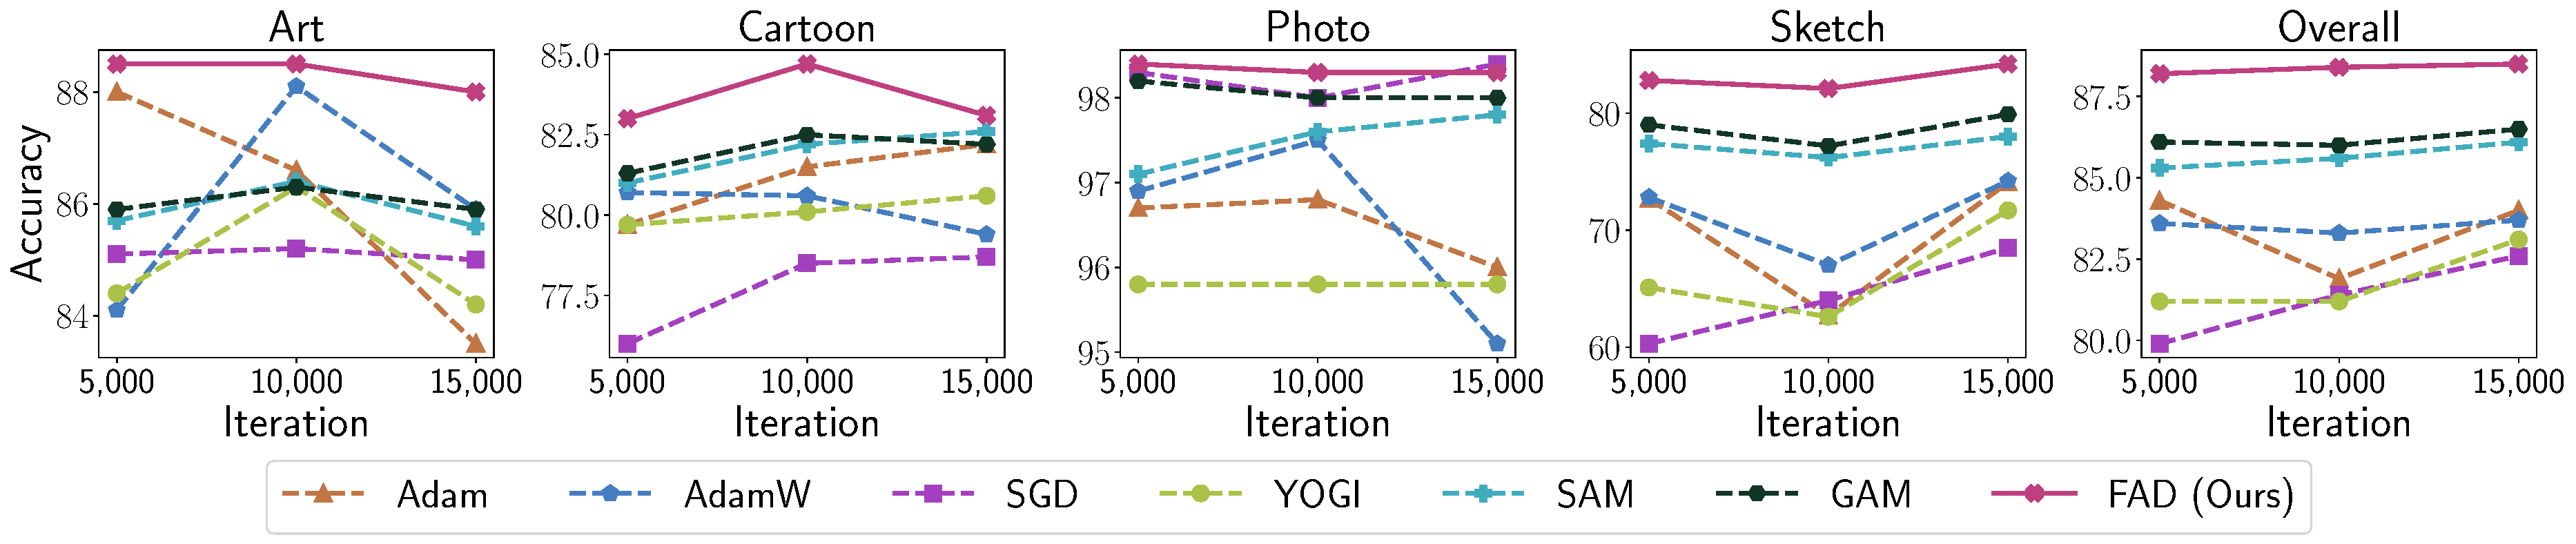
\includegraphics[width=\linewidth]{figs/iter_PACS.pdf}
    \caption{Accuracy of different methods on PACS with different training iterations.}
    \label{fig:iter_pacs}
\end{figure}

\begin{figure}[t]
    \centering
    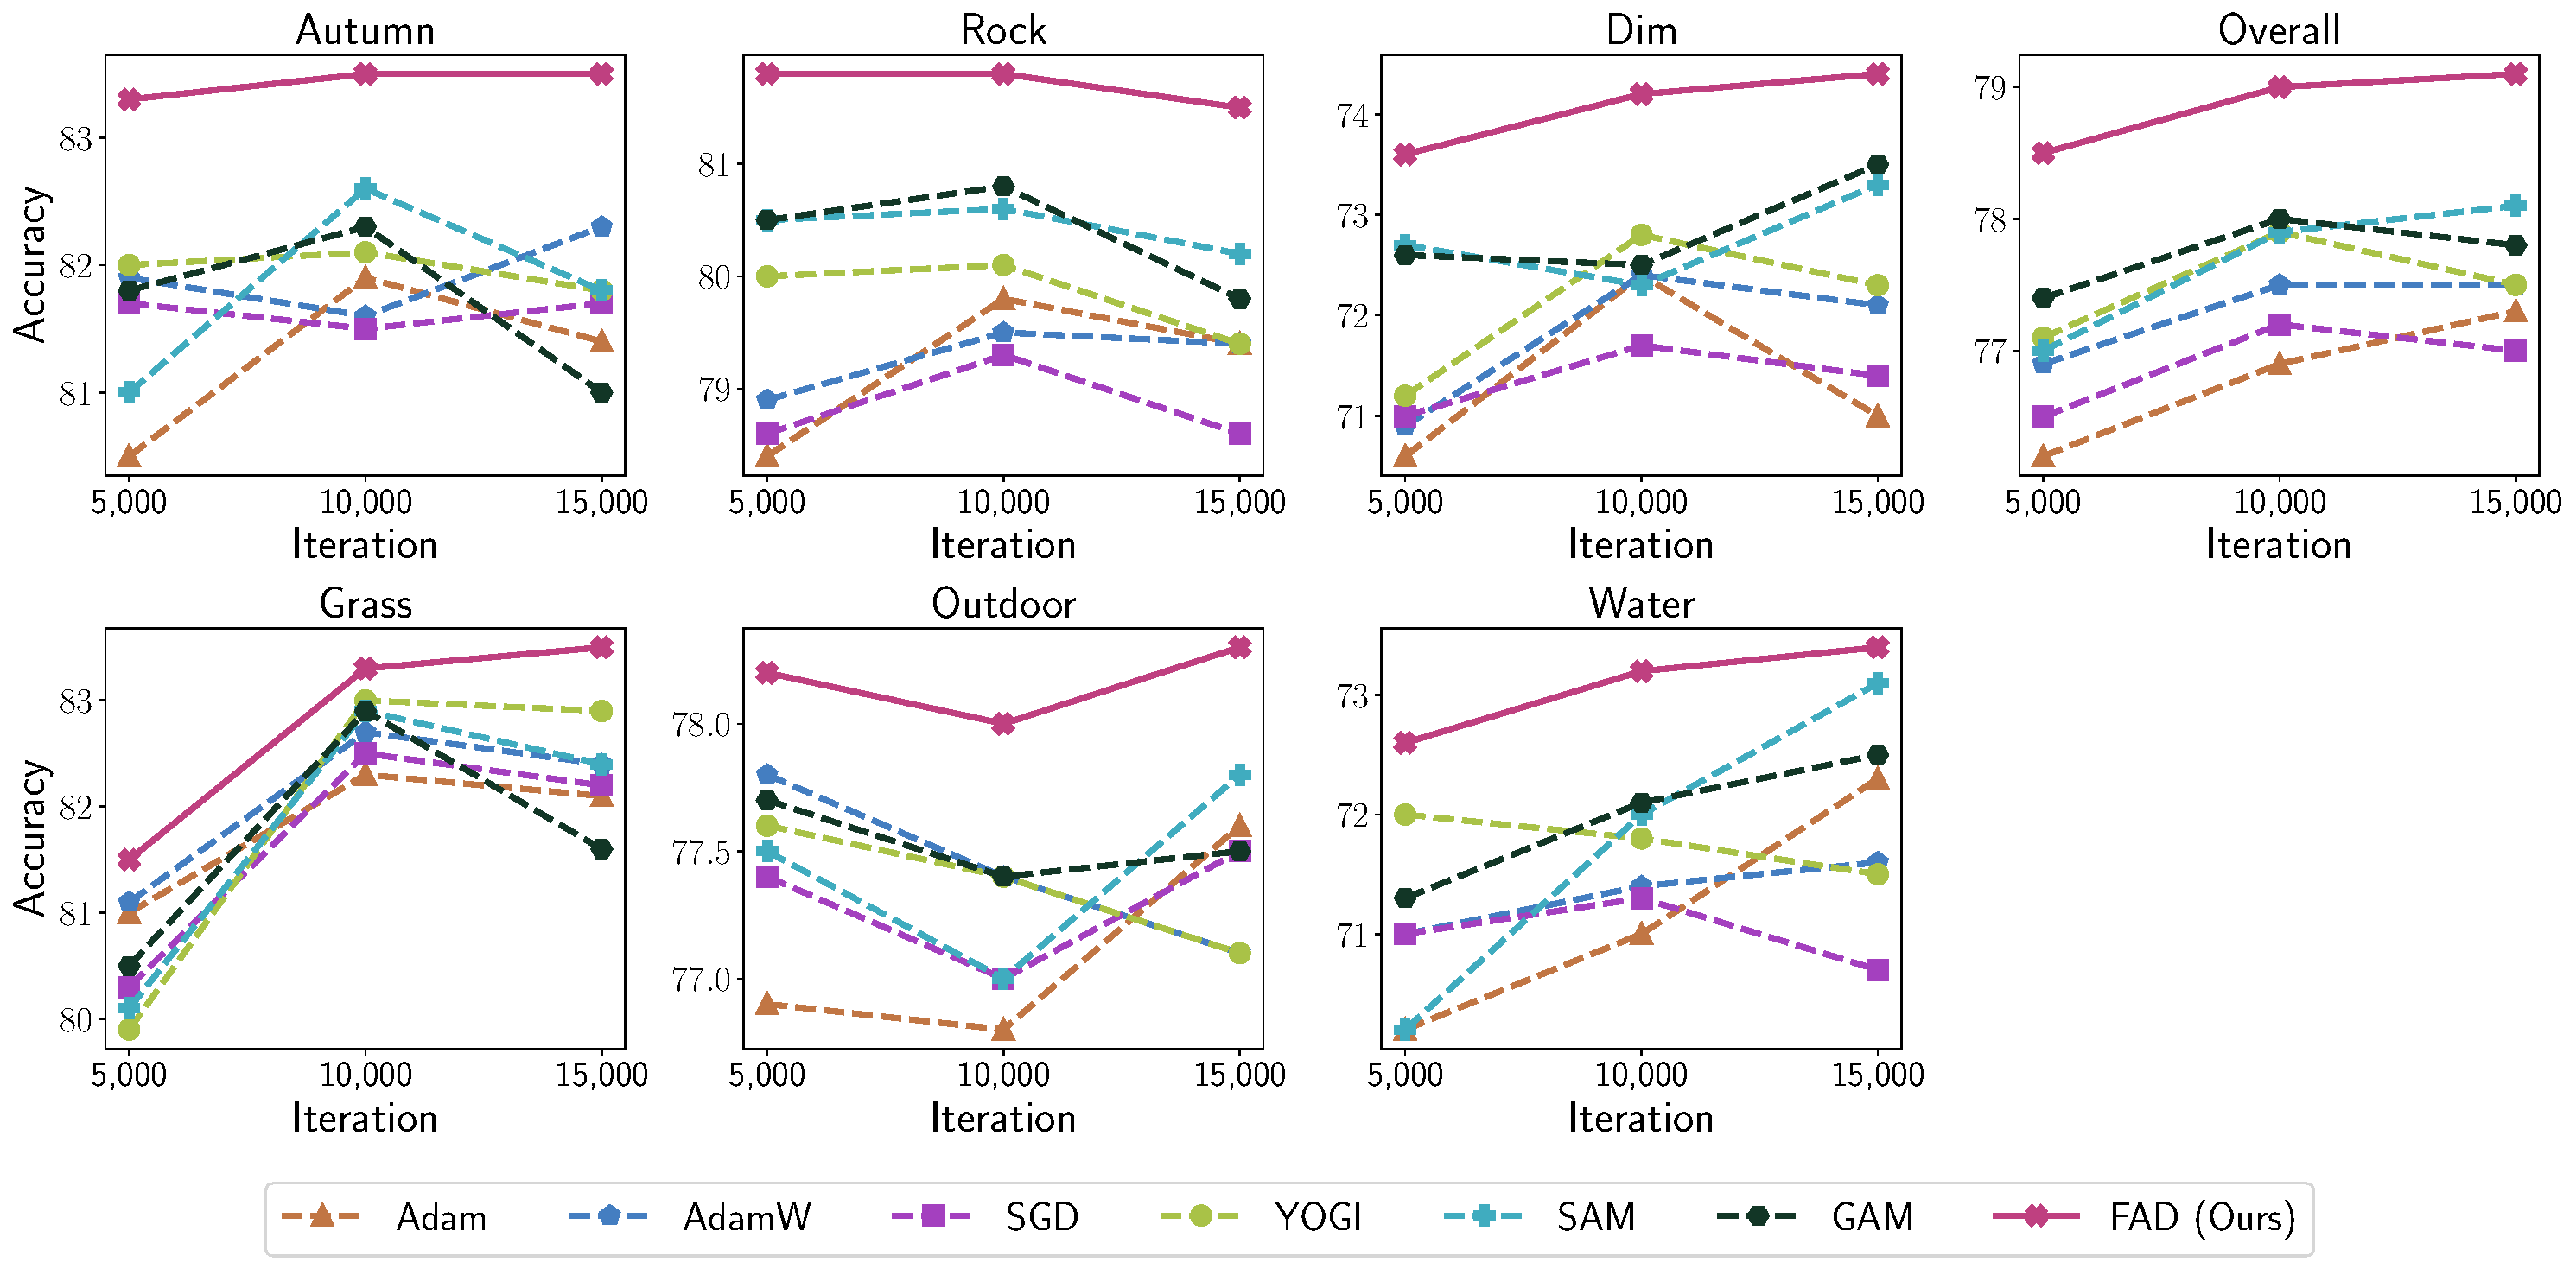
\includegraphics[width=\linewidth]{figs/iter_NICO++.pdf}
    \caption{Accuracy of different methods on NICO++ with different training iterations.}
    \label{fig:iter_nico++}
\end{figure}

We show the results of models trained with current optimizers and FAD for various iterations on PACS and NICO++ in Figure \ref{fig:iter_pacs} and Figure \ref{fig:iter_nico++}, respectively. 
\subsubsection{Optimizers with more training iterations on PACS}
We report the detailed results on PACS trained with 10,000 iterations in Table \ref{tab:pacs10k}. FAD consistently outperforms its counterparts on all domains.

\begin{table*}[th]

\centering
\caption{The comparison of optimizers on PACS with 10,000 iterations.}
\begin{tabular}{lcccc|c}
\toprule
\textbf{Algorithm} & art & cartoon & photo & sketch  & \textbf{Avg.} \\
\midrule

Adam  & 86.6 &  81.5 & 96.8 & 62.7 & 81.9\\
AdamW  & 88.1 & 80.6  & 97.5 & 67.0 & 83.3 \\
SGD  & 85.2 & 78.5  & 98.0 & 64.0 & 81.4 \\
YOGI  & 86.3 & 80.1  & 95.8 & 62.6 & 81.2 \\
SAM  & 86.4 & 82.2 & 97.6 & 76.2 & 85.6 \\
GAM  & 86.3 & 82.5  & 98.0 & 77.2 & 86.0 \\

\midrule
FAD (ours) & \textbf{88.5}  & \textbf{84.7}   & \textbf{98.3}& \textbf{82.1}  & \textbf{88.4} \\

\bottomrule
\end{tabular}
\label{tab:pacs10k}
\end{table*}

We report the detailed results on PACS trained with 15,000 iterations in Table \ref{tab:pacs15k}. FAD consistently outperforms its counterparts on all domains.
\begin{table*}[th]
\centering
\caption{The comparison of optimizers on PACS with 15,000 iteration.}
\begin{tabular}{lcccc|c}
% 
\toprule
\textbf{Algorithm} & art & cartoon & photo & sketch  & \textbf{Avg.} \\
\midrule

Adam  & 83.5  & 82.2 & 96.0 & 74.1 & 84.0 \\
AdamW  & 85.9  & 79.4  & 95.1 & 74.2 & 83.7 \\
SGD  & 85.0 & 78.7  & 98.4 & 68.5 & 82.6 \\
YOGI  & 84.2 & 80.6  & 95.8 & 71.7 & 83.1 \\
SAM  & 85.6 & 82.6  & 97.8 & 78.0 & 86.1 \\
GAM  & 85.9 &  82.2 & 98.0 & 79.9 & 86.5 \\

\midrule
FAD (ours) & \textbf{88.0} & \textbf{83.1}   & \textbf{98.3} & \textbf{84.2}  & \textbf{88.5} \\

\bottomrule
\end{tabular}
\label{tab:pacs15k}
\end{table*}


\subsubsection{Optimizers with more training iterations on NICO++}
We report the detailed results on NICO++ trained with 5,000 iterations in Table \ref{tab:nico5k}. FAD consistently outperforms its counterparts on all domains.

\begin{table*}[th]
\centering
\caption{The comparison of optimizers on NICO++. All the models are trained for 5,000 iterations and evaluated following the protocol in DomainBed~\cite{gulrajani2020search}. The best results for each domain are highlighted in bold font.}
\begin{tabular}{lcccccc|c}
\toprule
\textbf{Algorithm} & Autumn & Rock & Dim & Grass  & Outdoor & Water &\textbf{Avg.} \\
\midrule

Adam  & 80.5 & 78.4 & 70.6 & 81.0 & 76.9 & 70.2 & 76.2 \\
AdamW  & 81.9 & 78.9  & 70.9 & 81.1 & 77.8 & 71.0 & 76.9 \\
SGD  & 81.7 & 78.6 & 71.0 & 80.3 & 77.4 & 71.0 & 76.5 \\
YOGI  & 82.0 & 80.0 & 71.2 & 79.9 & 77.6 & 72.0 & 77.1 \\
SAM  & 81.0 & 80.5  & 72.7 & 80.1 & 77.5 & 70.2 & 77.0\\
GAM  & 81.8 & 80.5  & 72.6 & 80.5 & 77.7 & 71.3 & 77.4\\
\midrule
FAD (ours)  &  \textbf{83.3} & \textbf{81.8}   & \textbf{73.6}  & \textbf{81.5}  & \textbf{78.2}  & \textbf{72.6}  &  \textbf{78.5}\\

\bottomrule
\end{tabular}
\label{tab:nico5k}
\end{table*}

We report the detailed results on NICO++ trained with 15,000 iterations in Table \ref{tab:nico15k}. FAD consistently outperforms its counterparts on all domains.

\begin{table*}[th]
\centering
\caption{The comparison of optimizers on NICO++. All the models are trained for 15,000 iterations and evaluated following the protocol in DomainBed~\cite{gulrajani2020search}. The best results for each domain are highlighted in bold font.}
\begin{tabular}{lcccccc|c}
\toprule
\textbf{Algorithm} & Autumn & Rock & Dim & Grass  & Outdoor & Water &\textbf{Avg.} \\
\midrule

Adam  & 81.4 & 79.4 & 71.0 & 82.1  & 77.6 & 72.3  &  77.3\\
AdamW  & 82.3 & 79.4 & 72.1 & 82.4  & 77.1 & 71.6 & 77.5 \\
SGD  & 81.7 & 78.6 & 71.4 & 82.2 & 77.5 & 70.7 & 77.0 \\
YOGI  & 81.8 & 79.4 & 72.3 & 82.9 & 77.1 & 71.5 & 77.5 \\
SAM  & 81.8 & 80.2 & 73.3 & 82.4 & 77.8 & 73.1 & 78.1 \\
GAM  & 82.0 & 79.8 & 73.5 & 81.6 & 77.5 & 72.5 & 77.8\\
\midrule
FAD (ours)  & \textbf{83.5} & \textbf{81.5} & \textbf{74.4}  & \textbf{83.5} & \textbf{78.3} & \textbf{73.4}  & \textbf{79.1} \\

\bottomrule
\end{tabular}
\label{tab:nico15k}
\end{table*}





\subsection{Ablation study}
\begin{figure}[t]
    \centering
    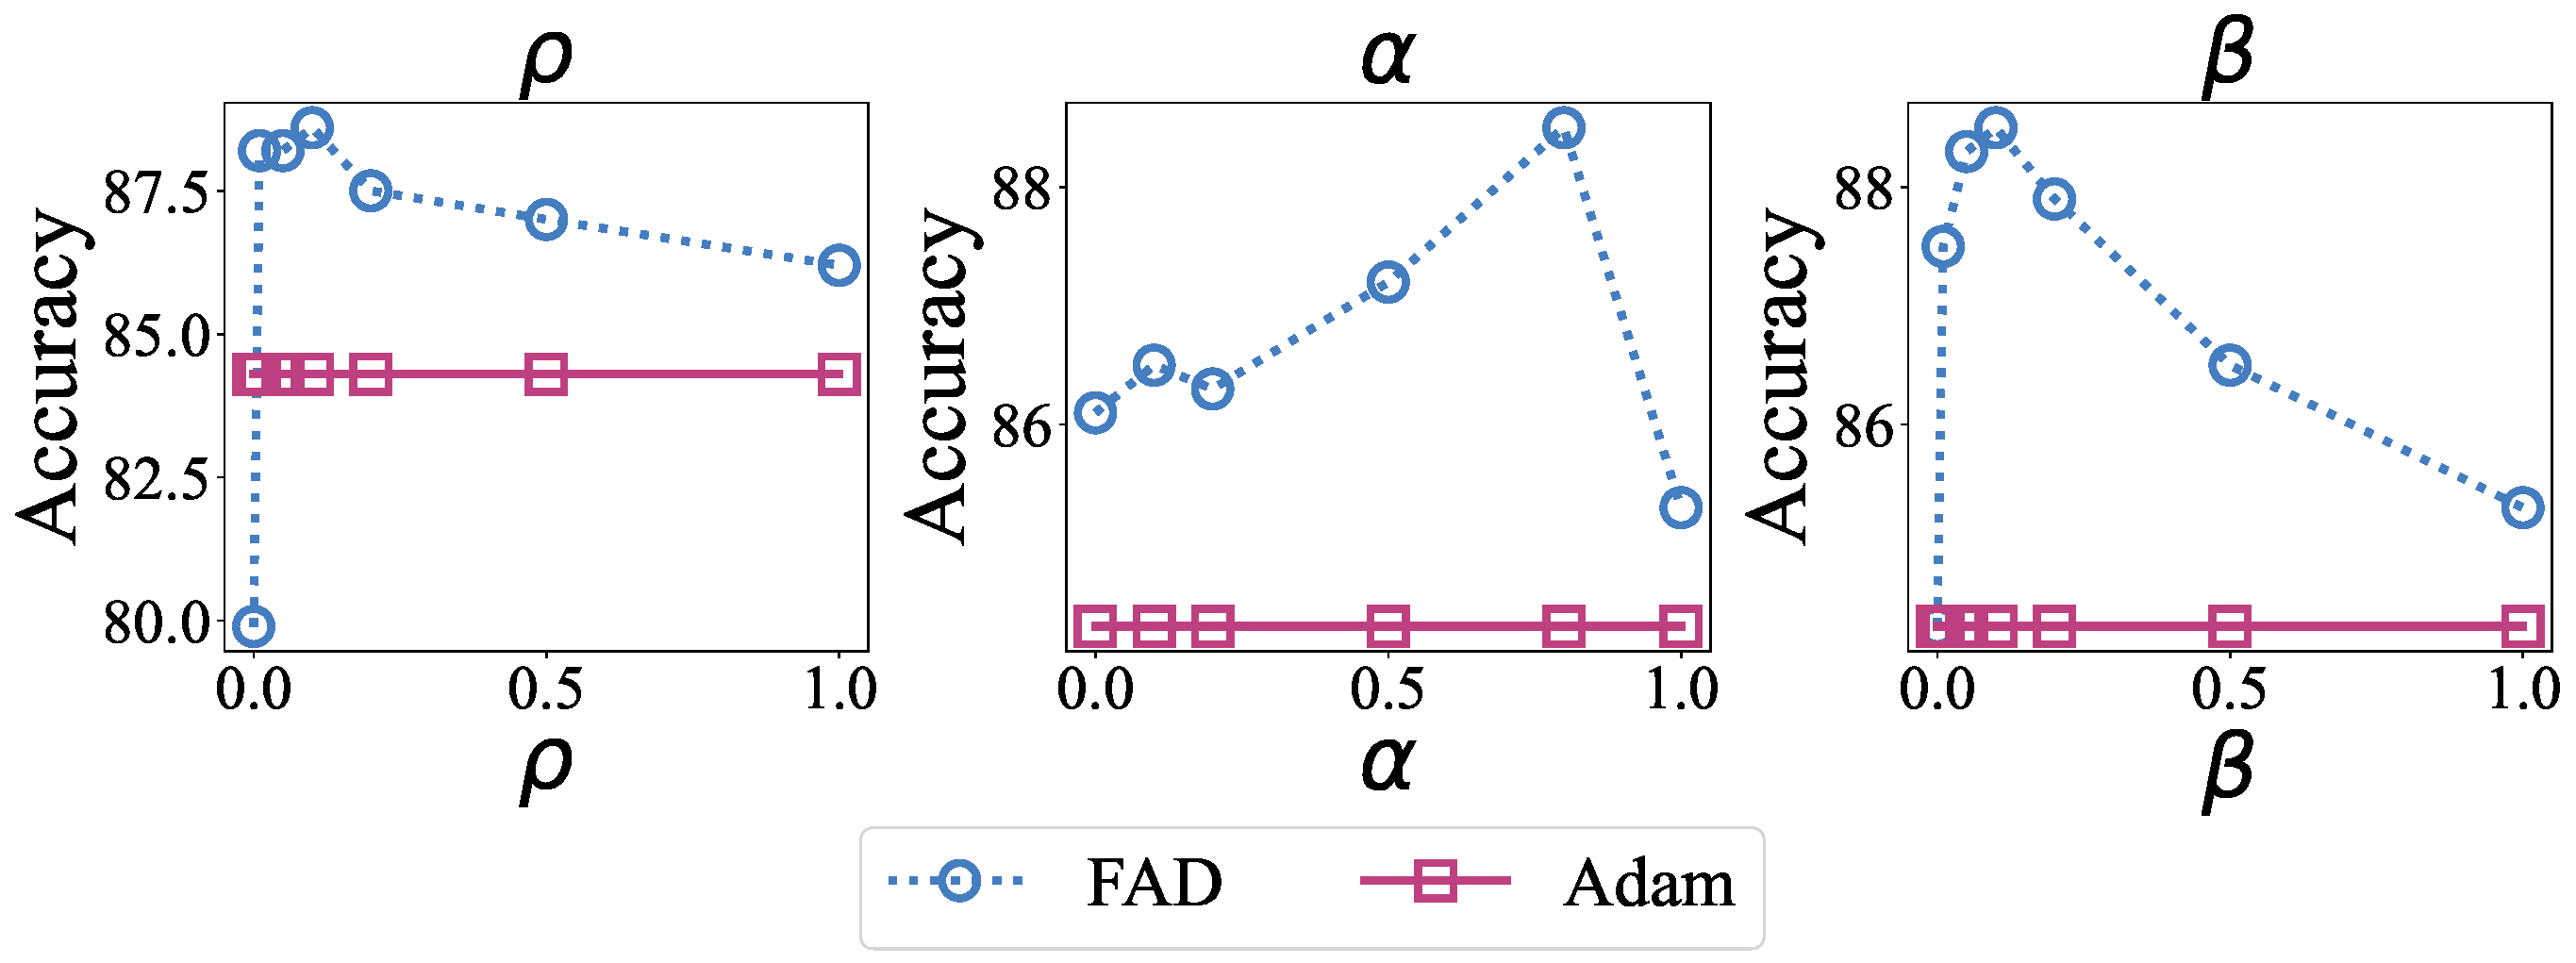
\includegraphics[width=0.9\linewidth]{figs/ablation.pdf}
    \caption{Accuracy of different methods on PACS with different training iterations.}
    \label{fig:ablation}
\end{figure}

FAD has three hyperparameters, namely $\rho$, $\alpha$, and $\beta$. Here we investigate the influence of the choice of them on PACS. The results are shown in Figure \ref{fig:ablation}. 
$\rho$ controls the step length of gradient ascent in FAD. When $\rho$ is set to 0, FAD degenerates into its base optimizer, i.e., SGD. When $\rho$ is larger than 0, FAD consistently outperforms SGD and Adam, as shown in the subfigure on the left of Figure \ref{fig:ablation}. $\alpha$ controls the proportion of intensity distributed between the zeroth-order and first-order flatness. When $\alpha$ is set to 0, FAD degenerates into GAM. Similarly, when $\alpha$ is set to 1, FAD degenerates into SAM. FAD consistently outperforms Adam with various choices of $\alpha$, as shown in the subfigure on the middle of Figure \ref{fig:ablation}. When $\beta$ is set to 0, FAD degenerates into its base optimizer, i.e., SGD. When $\beta$ is larger than 0, FAD consistently outperforms SGD and Adam, as shown in the subfigure on the right of Figure \ref{fig:ablation}. Please note that we only conduct grid search for the ablation study, the hyperparameters in other experiments are chosen based on the validation performance instead of test performance following the protocol in DomainBed. During the training and model selection phase, the information pertaining to the test data is not available.